\documentclass{report}

\usepackage[utf8]{inputenc}
\usepackage[export]{adjustbox}
\usepackage[a4paper, top=2.5cm, bottom=2.5cm, left=2.2cm, right=2.2cm]
{geometry}

\usepackage{graphicx}
\usepackage{gensymb}
\usepackage{float}
\usepackage[export]{adjustbox}
\usepackage{wrapfig}
\usepackage{subcaption}

%\includegraphics[opciones]{ruta}

\title{Climatología en Puerto Libertad} % Asignamos un título al documento

\author{Paul Maximiliano Rivera Medina\\
    \\
    Departamento de Física \\
    Universidad de Sonora} 

\date{15 enero de 2021} 

\begin{document}

\maketitle

\section{Introducción}
El pronostico del clima, es algo maravilloso si se ve a fondo. El calculo del mismo conlleva muchas variables, que bien podríamos englobarlas en tres tipo: geográficos, atmosféricos, termodinámicos. La obtención de estos valores se realiza por distintos medios. Los geográficos no resultan mucho problema con la información obtenida de una cuadrilla o más (dependiendo la extinción del terreno) es suficiente por muchos años. En cambio los otros dos tipos de datos son muy irregulares a lo largo del tiempo por eso es necesario actualizarlos constantemente.Las estaciones meteorológicas, son las encargadas de la recabar la información necesaria para cubrir estos dos rubros, estas son colocadas a lo largo de todo el país, hay regiones con mas de una. Individualmente todas pueden dar buenos resultados en su posición, pero estas trabajan en conjunto para mejorar la precisión y abarcar fenómenos que afecten a mas de una zona.

\section{Antecedentes}
La estación de la cual se han recabado los presentes datos es la numero 26071 localizada en Puerto Libertad, una localidad y puerto del estado mexicano de Sonora, situado en la costa norte del Golfo de California, en el municipio de Pitiquito. Puerto Libertad se encuentra localizado en las coordenadas geográficas 29°54'15''N 112°40'59''O y a una altitud de 13 metros sobre el nivel del mar. Esta estación cuenta con 48 años de datos.

\section{Datos}

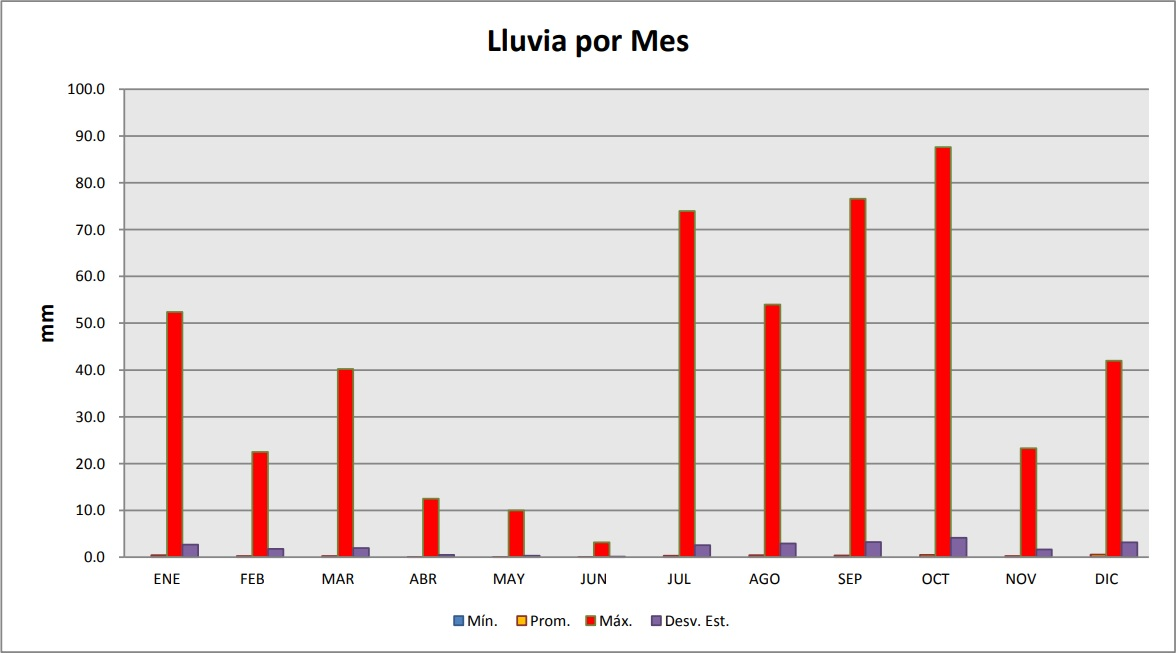
\includegraphics[width=0.9\linewidth]{1.jpg}
\\
\\
\noindent
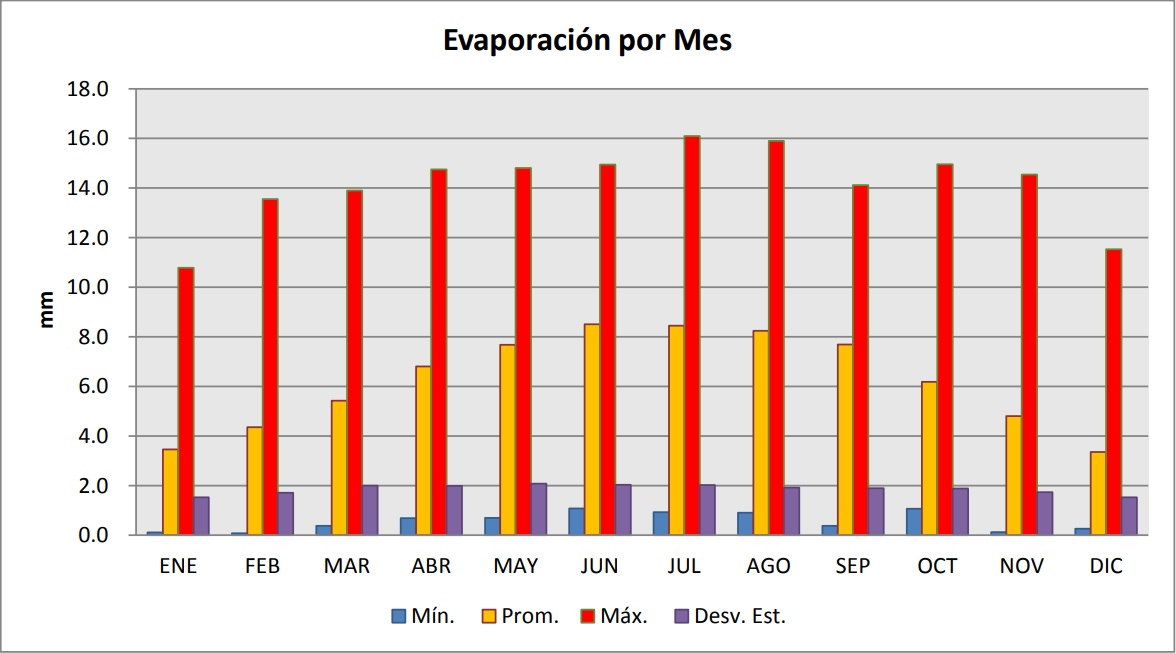
\includegraphics[width=0.9\linewidth]{2.jpg}
\\
\noindent
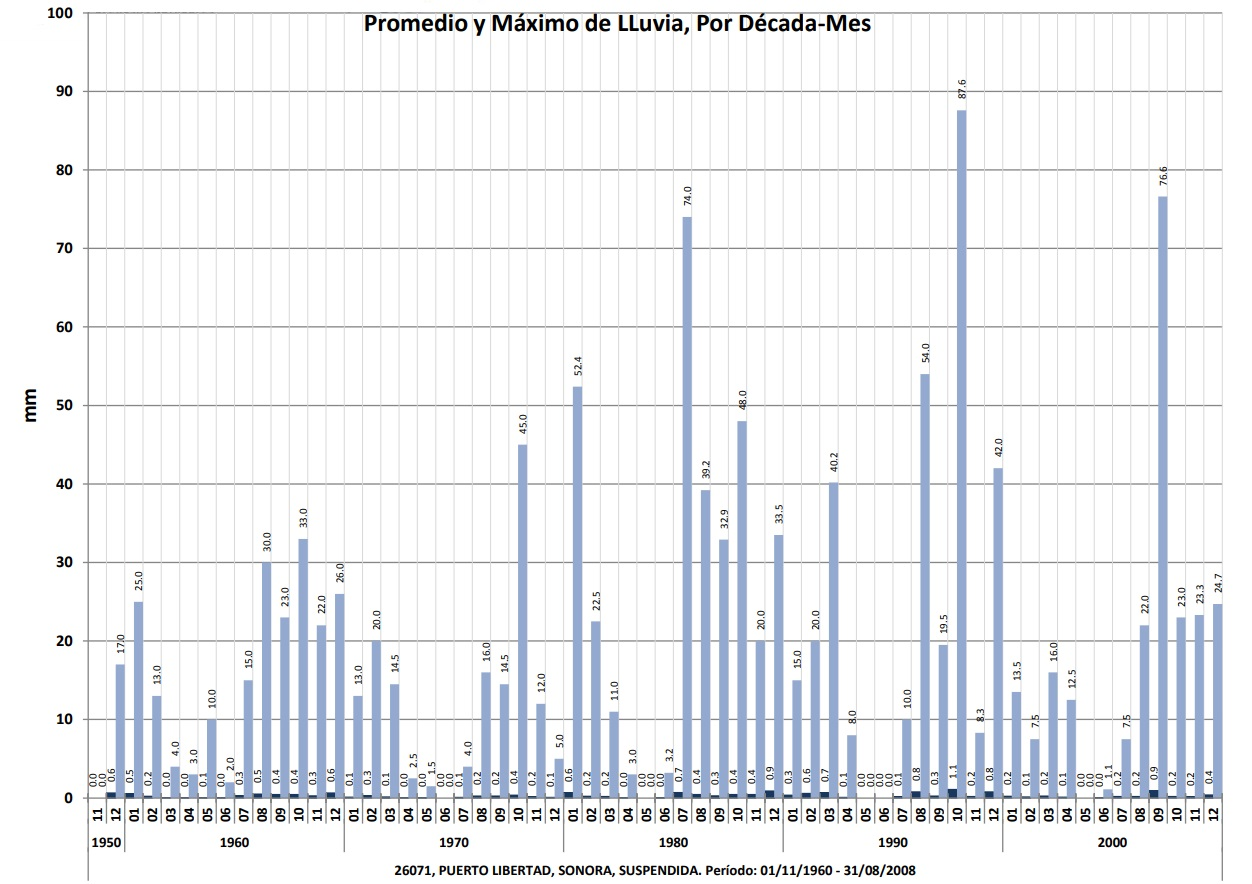
\includegraphics[width=0.9\linewidth]{3.jpg}
\\
\noindent
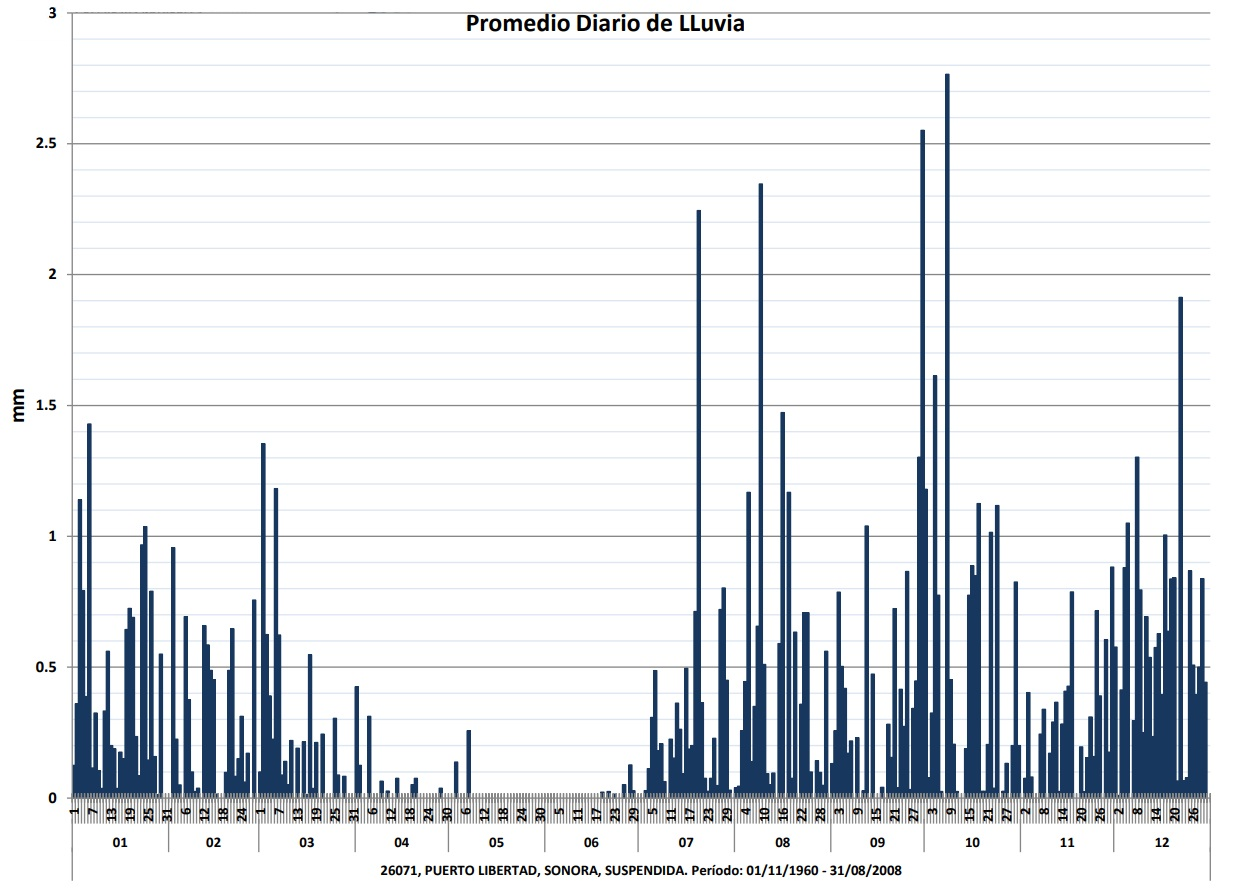
\includegraphics[width=0.9\linewidth]{4.jpg}
\\
\noindent
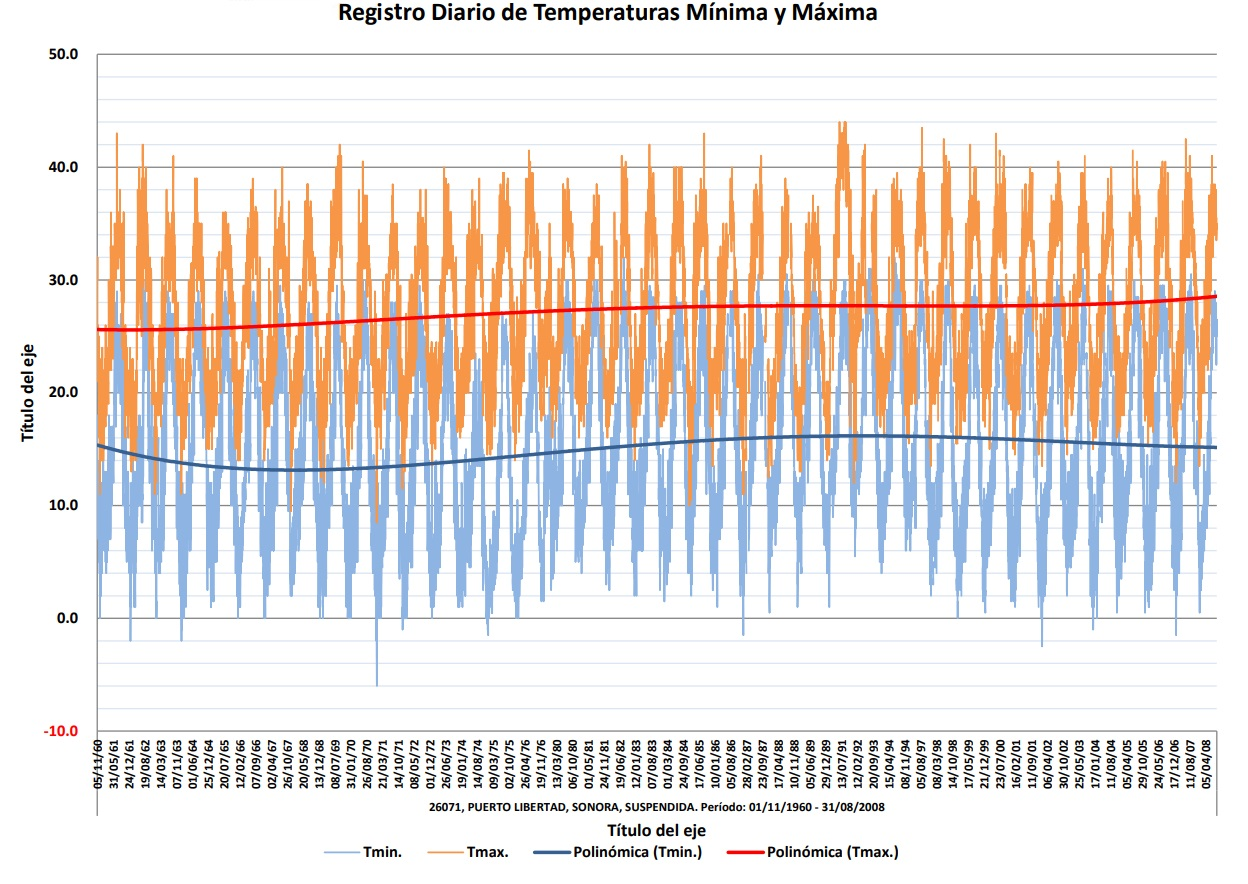
\includegraphics[width=0.9\linewidth]{5.jpg}
\\
\noindent
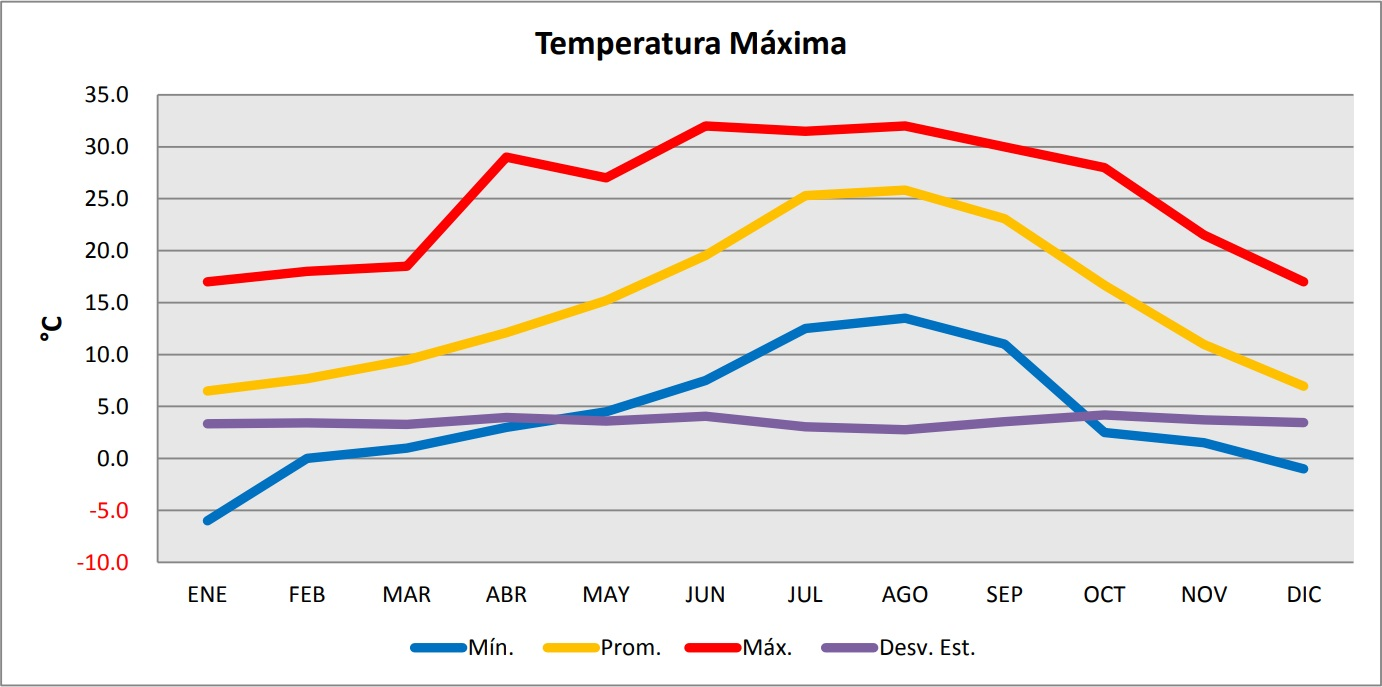
\includegraphics[width=0.9\linewidth]{6.jpg}
\\
\noindent
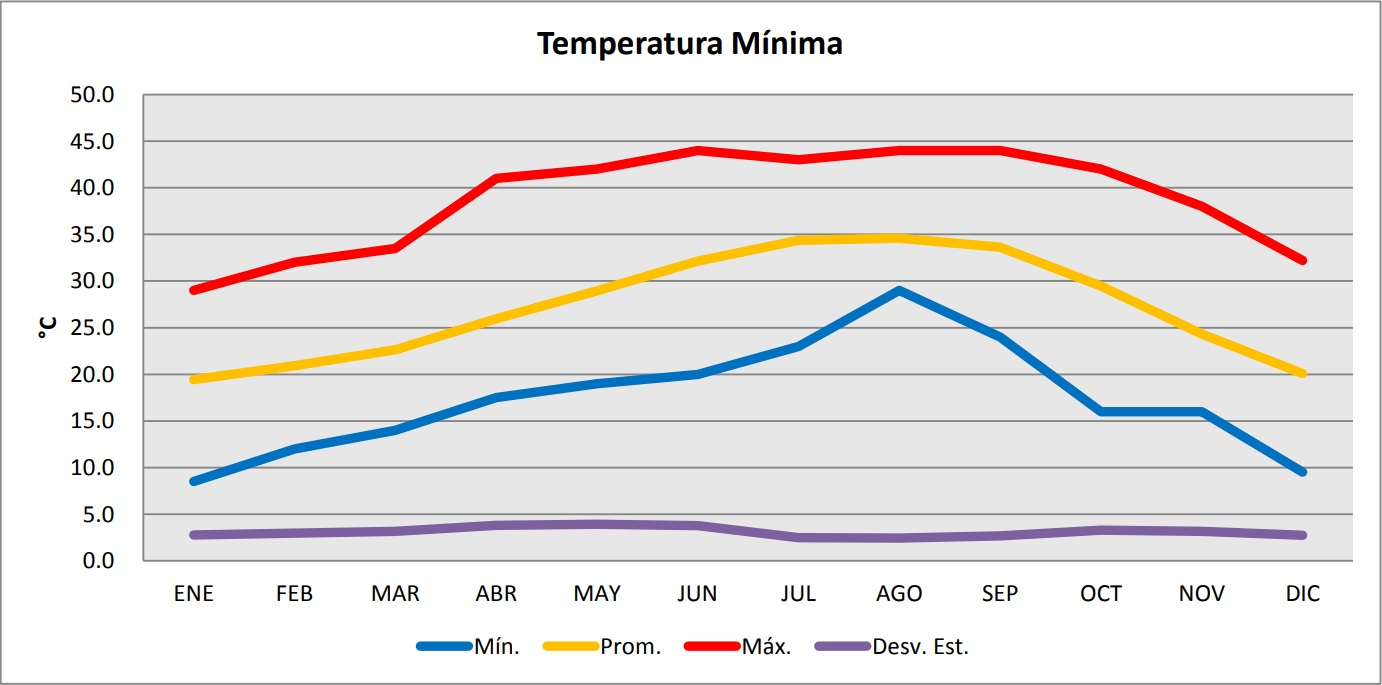
\includegraphics[width=0.9\linewidth]{7.jpg}

\section{Conclusión}
Puerto libertad es una zona en la que llueve muy poco, promedio de lluvias por mes menores a 2. Tiene una evaporaciones promedio de 5mm por mes. La mayor lluvia registrada por esta estación fue en la década de los 90 con 87.6 mm. Una temperatura máxima media de 27.5°C . siendo esta una zona desértica son muchas lluvias pero no es extrañar siendo un puerto.

\section{Apéndice}

\begin{enumerate}
\item \textbf{¿Qué te pareció?}\\
\textit{Apropiada, si \LaTeX es lo que usaremos toda la vida profesional entre mas rápido empezamos mejor}
\item \textbf{¿Cómo estuvo el reto?}\\
\textit{sencillo, para hacerlo en cinco días, demasiado fácil }
\item \textbf{¿Qué se te dificultó más?} \\
\textit{El acomodo de las gráficas, al poner el tipo reporte en "documentclass" pensé que daría todo el formato, pero después de muchos intentos ya quedaron acomodadas}
\item \textbf{¿Qué te aburrió?}\\
\textit{El tema, para los objetivos de la actividad es irrelevante, pero tiene que tener introducción así que hay que cumplir}
\item \textbf{¿Qué recomendarías para mejorar la primera Actividad?}\\
\textit{Hacer las gráficas uno mismo, con el software de preferencia de cada quien, para que algunos(la minoría) empezamos  a usar R o algo parecido,pero otro tema porque si ya están se siente un poco raro al hacerlo}
\item \textbf{¿Que grado de complejidad le asignarías a esta Actividad?} \\
\textit{En general, de introducción, no hay parámetros a los cuales apegarnos y eso facilita la culminación de la actividad}

\end{enumerate}

\end{document}
